% vim: ft=tex
\chapter{Requirements}\label{ch:reqs}
The requirements gathered during the first and second meeting with the client are
explained in this chapter. These are more concrete than the ones listed in the
Task Description in \autoref{ch:task-desc}.

First of all, these are the client's priorities:

\begin{enumerate}
\item Federation functionality, namely:
	\begin{enumerate}
		\item Topology definition
		\item DIM synchronization
		\item Message routing
	\end{enumerate}
\item \Gls{HA}
\item Persistence synchronization
\item Encryption (optional)
\item DIM access control
\item OPC UA \gls{HA} (optional)
\end{enumerate}

The following sections explain the requirements in greater detail, starting
with the functional ones. The non-functional requirements are described in
\autoref{sec:nfr}.

The functional requirements are each described in prosa as understood by the
students first and then formally in \gls{gherkin} style features. Those feature
specifications will later be useful to deduce test cases.

\section{Federation}
Roadster will need to be run on multiple nodes in a hierarchical topology,
forming a distributed computing architecture. The root node would then act as
the client-facing server. Typical node topologies include:

\begin{description}
	\item [ Single level, single node ] \hfill\\
		This is the legacy setup and is what Roadster is already able
		to do. It consists of a single node. This is illustrated in
		\autoref{fig:topo:sl:noha}.

	\item [ Multi level ] \hfill\\
		This is the most basic federation setup. There is a root node, and
		two subnodes. Each subnode is directly connected to a number of field devices such as
		\glspl{PLC} or emergency phones. This is illustrated in
		\autoref{fig:topo:ml:noha}.
\end{description}

\begin{figure}[]
	\center
	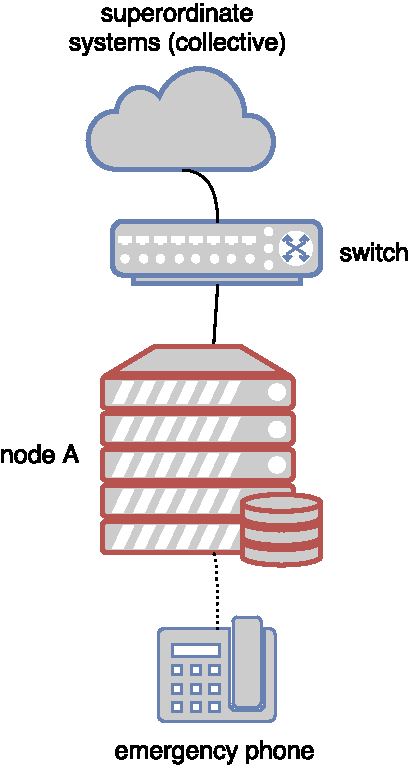
\includegraphics[width=0.25\textwidth]{img/topo_sl_noha.pdf}
	\caption{Physical legacy example: a single node and a field device each}
	\label{fig:topo:sl:noha}
\end{figure}
\begin{figure}[]
	\center
	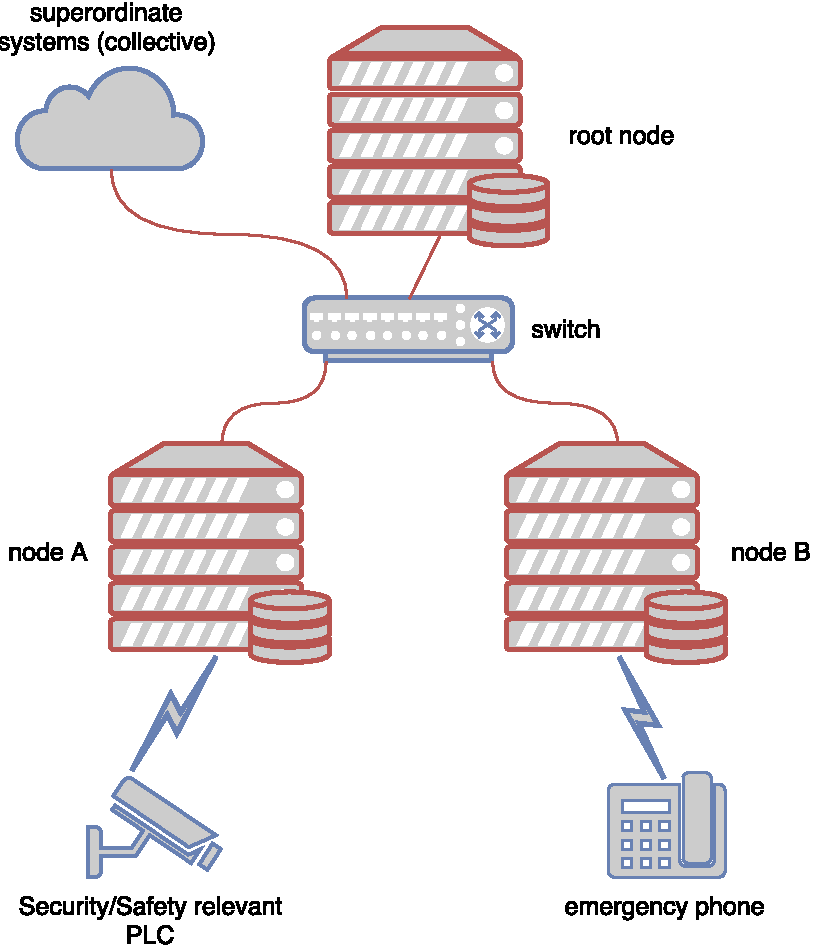
\includegraphics[width=0.5\textwidth]{img/topo_ml_noha.pdf}
	\caption{Physical federation topology example: supernode, two subnodes, a field device each}
	\label{fig:topo:ml:noha}
\end{figure}

This is formally specified in \autoref{lst:feature:federation}

\begin{listing}
	\inputminted{Gherkin}{listings/features/federation/federation.feature}
	\caption{Formal federation feature}
	\label{lst:feature:federation}
\end{listing}

\subsection{DIM extension}

\subsubsection{Synchronization}
Extending the \gls{CSP} to keep the \gls{DIM} consistent across all nodes is a central
part of the federation functionality. This means replicating modifications to
the dynamic DIM objects to all other actors on the node (legacy behavior) and
to all other nodes.

\paragraph{Duplex.} Unlike the CSP, it needs to go both ways. The server won't
be the single source of truth. Every node will be responsible for part of the
DIM, thus it will have to inform its neighbors about modifications that have
happend in the meantime, no matter if the neighbor node in question is a
supernode or a subnode.

According to the meta model in \autoref{fig:roadster:meta-model}, these dynamic
objects are exactly the instances of one of the following three
classes (marked yellow in the class diagram):
\begin{itemize}
	\item \rb{DataItem}
	\item \rb{Session}
	\item \rb{Case}
\end{itemize}

As described earlier, instances of these entity classes are marked "dirty" when
modified until they are replicated.

\subsubsection{Access control}
The above requirements imply that modifications to the \gls{DIM} can only be done by the
owning node. A node
must not modify objects owned by other nodes directly. This is to ensure that each node is its own source of truth
to all other nodes in the federation. Only the owner node can enforce a single
sequence of updates to its part of the DIM, which is necessary to guarantee
eventual consistency \cite[Chapter 5, Reliable Pub-Sub (Clone Pattern), Republishing
Updates from Clients]{zmq:zguide} across all actors of all nodes.

These two aspects to the DIM extension are formally specified in \autoref{lst:feature:federation:dimsync}

\begin{listing}
	\inputminted{Gherkin}{listings/features/federation/dim_extension.feature}
	\caption{Formal DIM synchronization feature}
	\label{lst:feature:federation:dimsync}
\end{listing}

\subsection{Autonomy}
It's important that every node (and its subnodes) can keep up the operation autonomously even if the
link to its supernode fails or the supernode itself fails. This means that updates to
the \gls{DIM} must be possible even when neighboring nodes (including the supernode) are unavailable. After the
recovery from the outage, the \gls{DIM} synchronization shall be reinitiated so
all pending updates are shared to all other nodes as per normal operation.

This is formally specified in \autoref{lst:feature:federation:autonomy}

\begin{listing}
	\inputminted{Gherkin}{listings/features/federation/autonomy.feature}
	\caption{Formal autonomy feature}
	\label{lst:feature:federation:autonomy}
\end{listing}

\subsection{Message routing}
There needs to be a message routing mechanism so a user
of one node's web UI can send a command (passed as a message) to another node where it will be
executed. An example for this is a forced value in the DIM to ignore the
actually measured value reported by a device in case the device is known to be
wrong. The common case where the command is issued at a higher level in the node
topology is priority. E.g. in a setup with a root node and two
subnodes A and B, issuing a command on A for B has a low priority.

This is formally specified in \autoref{lst:feature:federation:cmdrouting}

\begin{listing}
	\inputminted{Gherkin}{listings/features/federation/message_routing.feature}
	\caption{Formal message routing feature}
	\label{lst:feature:federation:cmdrouting}
\end{listing}

\section{High availability}
Roadster must be able to run in certain high availability setups. Achieving
this is done by adding redundant Roadster nodes.

The following additional federation topologies must be supported:
\begin{description}
	\item [ Single level \gls{HA} ] \hfill\\
		This is when there are exactly two nodes, both of them
		connected to the same set of field devices. The difference to a
		non-redundant case is the added backup node, forming a HA
		cluster. The field devices are thus connected to the HA cluster
		using two redundant paths. Both HA peers are able to interact
		with the field devices to perform operation tasks (e.g. reading
		sensor data, writing down configurations), but only one of them
		(the active one) must do so. This is illustrated in
		\autoref{fig:topo:sl:ha}.

	\item [ Multi level, \gls{HA} at root only ] \hfill\\
		There can be multiple hierarchy levels within a Roadster federation, such as two or
		three (anything else is considered exotic). Introducing
		redundancy is done at the root level in the form of a HA
		cluster, consisting of a primary and a backup node. An example of this setup is illustrated in
		\autoref{fig:topo:ml:ha}.
\end{description}

\begin{figure}[]
	\center
	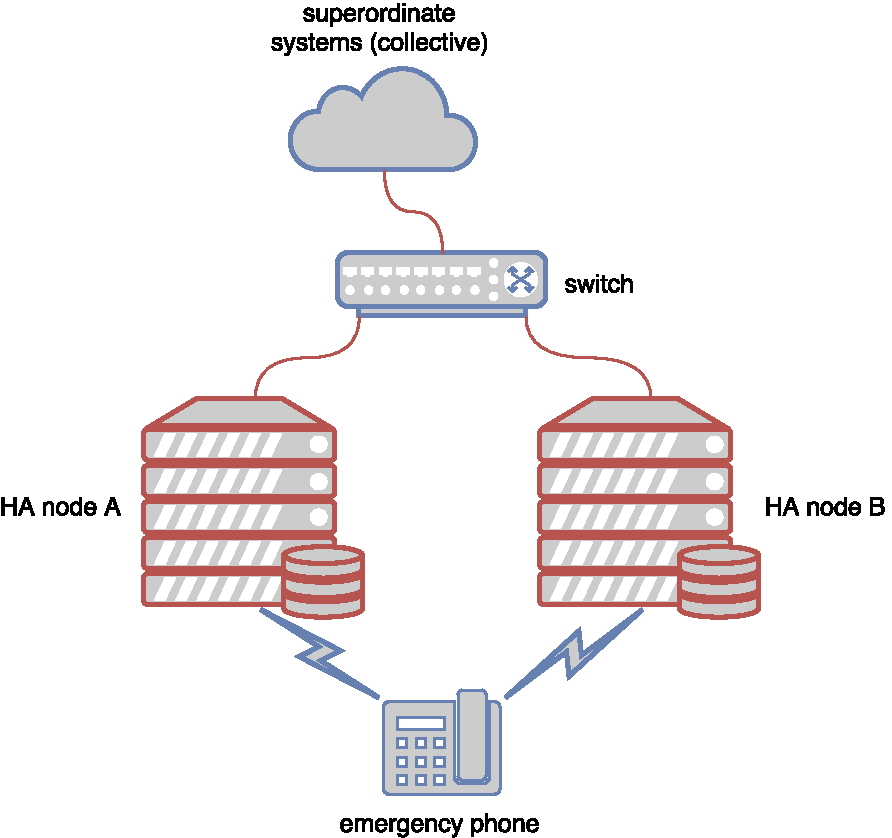
\includegraphics[width=0.5\textwidth]{img/topo_sl_ha.pdf}
	\caption{Federation example: a HA cluster and redundantly connected field devices}
	\label{fig:topo:sl:ha}
\end{figure}
\begin{figure}[]
	\center
	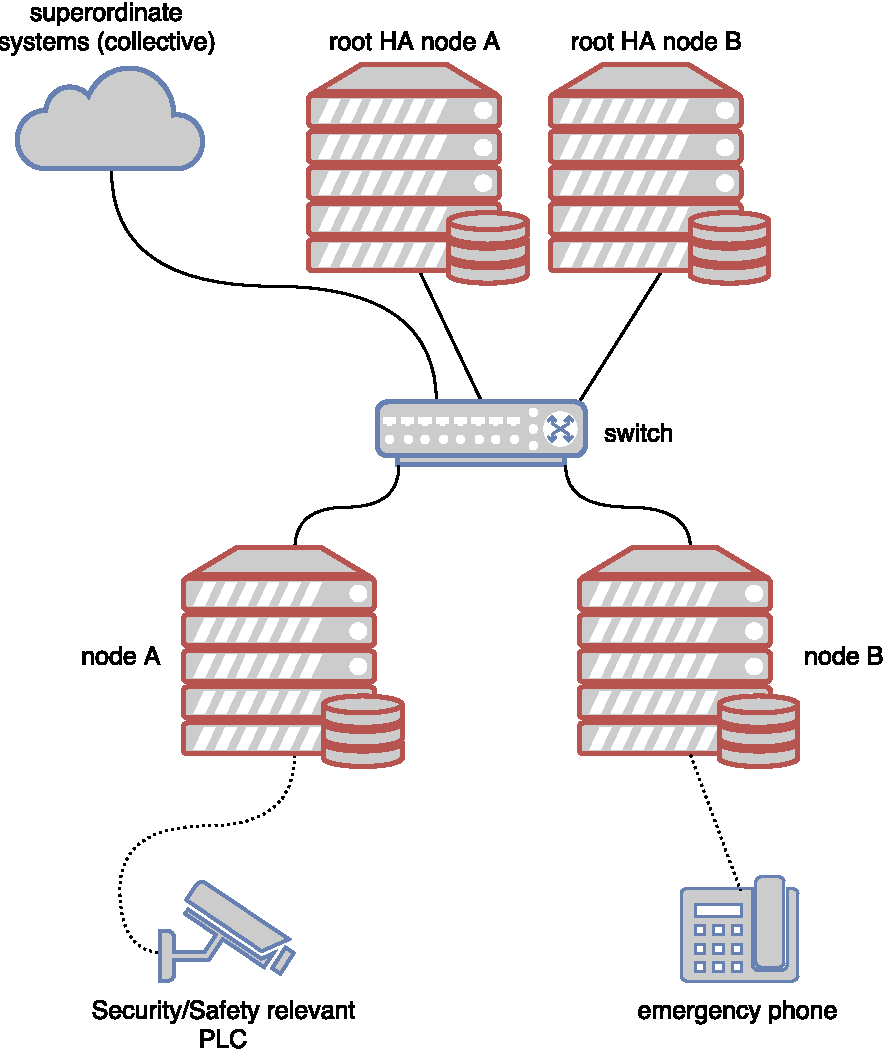
\includegraphics[width=0.5\textwidth]{img/topo_ml_ha.pdf}
	\caption{Federation example: HA cluster at root, two subnodes, each with field devices}
	\label{fig:topo:ml:ha}
\end{figure}

The following cases are more exotic and are outside the scope of this thesis;
however, they should be kept in mind so a future extension to support them is
feasible:

\begin{description}
	\item [ Multi level, \gls{HA} at bottom ] \hfill\\
	A single root node at the top and a subordinate HA pair each connected
	to the same field device.

	\item [ Multi level, \gls{HA} in the middle ] \hfill\\
	A single root node at the top, a subordinate HA pair, which in turn has
	a subordinate node connected to some field device.
\end{description}


\paragraph{Dedicated network link.}
It's possible that there's a dedicated, direct network link from one peer to
the other. However, this won't be typical.

\paragraph{Split-brain syndrome.}
At initialization, the two peers must automatically find consensus on which one
is becomes active first.  At any time, only one of the two HA peers must be
active (i.e. serving clients), and the other one must stay passive (i.e. ignore
client requests and only keep its DIM up-to-date). The passive HA peer shall
take over in the event that the currently active peer becomes unavailable.
Measures must be taken to avoid the dreaded split-brain syndrome where both HA
peers become active.

The types of failures that need to be handled include:
\begin{itemize}
	\item Software failure on the primary node, like an application or OS crash
	\item Hardware failure on the primary node, like a defect power supply
	\item Failure of a network link, completely disconnecting a HA peer from the federation
\end{itemize}

All three failure types listed above can collectively be called \emph{crash},
as their effects are the same from the point of view of the whole federation.

The high availability requirement is formally specified in \autoref{lst:feature:ha}

\begin{listing}
	\inputminted{Gherkin}{listings/features/high_availability.feature}
	\caption{Formal high availability feature}
	\label{lst:feature:ha}
\end{listing}

\section{Persistence synchronization}
This is about the synchronization of persisted data, which is currently stored
in \gls{tc} databases on a Roadster node, one for each kind of data. With the federation functionality, this is
still true: Every node will have its own set of key-value stores. Changes to the persisted
data must flow from south to north (towards the root node), so the root
node can collect and maintain a replication of the persisted data of all
nodes within the federation, recursively.

Again, it's important that every node and its subnodes form an autonomous subsystem. So
in case the link to its supernode fails, it has to continue working. As soon as
the link is repaired, synchronization of the delta (changes to the data) can
be initiatd.

This is different from \gls{DIM} synchronization, as the DIM is shared across
all nodes and is a relatively small data structure holding merely the current state. The \gls{tc} databases
can possibly contain large amounts of data (in the hundreds of megabytes) and
are shared only towards the root node (thus "bubbling up").

This is formally specified in \autoref{lst:feature:persistence_synchronization}

\begin{listing}
	\inputminted{Gherkin}{listings/features/persistence_synchronization.feature}
	\caption{Formal persistence synchronization feature}
	\label{lst:feature:persistence_synchronization}
\end{listing}

% ---------------------------------------------------------------------------
\section{Non-functional requirements}\label{sec:nfr}
The following subsections elaborate on the non-functional requirements.

\subsection{Simplicity}
The two reoccuring patterns that surfaced during the requirements gathering
meeting were:

\begin{enumerate}
\item \gls{KISS} principle. Simplicity is favored, as experience shows that
	simpler systems are more stable, so complexity should be avoided if not
	absolutely necessary.

\item No premature optimization since it's the root of all evil.\footnote{Quote
	by Donald Knuth: ``Premature optimization is the root of all evil.''}
\end{enumerate}


\subsection{Testing}
Regarding testing, the following requirements exist:
\begin{itemize}
	\item the student's contributions are verified with unit tests
	\item use cases shall be integration tested in a close-to-reality setup, either automatically or manually
\end{itemize}

\subsection{Constraints for persistence synchronization}
100\% consistency is not an absolute requirement for persistence synchronization.
Nor is zero data loss an absolut requirement. However, it is mandatory that
updates make it to the root node within 30 seconds.

\subsection{High availability for OPC UA}
The high availability feature shall be design with \gls{opc-ua} in mind. It
should be easy to adapt it to the various kinds of server redundancy specified
in OPC-UA, including the transparent and non-transparent variants.

\subsection{Encryption}
\emph{This is optional. Also, this requirement has the lowest priority not
because it's insignificant, but because it's easy to enable transport level
security on \zmq sockets later on.}

The inter-node communication of a Roadster federation must be secured using
encryption. Recent versions of \zmq offer modern, authenticated encryption,
including server and client authentication (the latter is optional).
The client favors a solution where every communication partner (a node)
authenticates all its communication partners, and vice versa.

Since the \zmq binding used in the legacy version is unmaintained and doesn't
allow encryption, it has to be exchanged with a more appropriate library.

\subsection{Coding Guidelines}
The coding guidelines desired by the client are basically the ones written down
in the popular Ruby style guide \cite{rb:style-guide}, with the following
differences or special remarks:

\begin{itemize}
	\item method calls: only use parenthesis when needed, even with
		arguments (as opposed to
		\footnote{\url{https://github.com/bbatsov/ruby-style-guide\#method-invocation-parens}})
	\item 2 blank lines before method definition (slightly extending
		\footnote{\url{https://github.com/bbatsov/ruby-style-guide\#empty-lines-between-methods}})
	\item YARD API doc, 1 blank comment line before param documentation,
		one blank comment line before code (ignoring
		\footnote{\url{https://github.com/bbatsov/ruby-style-guide\#rdoc-conventions}})
	\item Ruby 1.9 symbol keys are wanted
		\begin{itemize}
			\item e.g. \rb{foo: "bar", baz: 42} instead of \rb{:foo => "bar", :baz => 42}, just like
			\footnote{\url{https://github.com/bbatsov/ruby-style-guide\#hash-literals}}
		\end{itemize}
	\item align multiple assignments so there's a column of equal signs
\end{itemize}
